\documentclass[a4paper,12pt,oneside]{book}%extreport
\usepackage{times} 
% \usepackage{multibib}
\usepackage{lipsum}
\usepackage{appendix}
\usepackage[shortlabels]{enumitem}
\usepackage{booktabs}
\usepackage{rotating} % Rotating table
\usepackage{hhline}
\usepackage{colortbl}
\usepackage{afterpage}
\usepackage{mathtools} %Fixes/improves amsmath
\usepackage{setspace}
\usepackage[utf8]{vietnam} 
\usepackage{amstext, amsmath,latexsym,amsbsy,amssymb, amssymb,amsthm,amsfonts,multicol, nccmath}
\usepackage[left=3cm,right=2cm,top=2.5cm,bottom=3cm,footskip=40pt]{geometry}
\usepackage{pdflscape}
\usepackage{apacite}
\usepackage{tikz}
\usepackage{array}
\newcolumntype{C}[1]{>{\centering\let\newline\\\arraybackslash\hspace{0pt}}m{#1}}
\usetikzlibrary{calc}
\usepackage{tabularx}
\usepackage{multicol}
\usepackage{array,color,colortbl}
\setcounter{secnumdepth}{4}
\usepackage{placeins}
 %\usepackage[square,numbers]{natbib}
\usepackage[square, comma, numbers, sort&compress]{natbib}
\setlength{\parindent}{1cm}
\usepackage{color}
\usepackage{indentfirst}
\usepackage{exscale,eucal}
\usepackage{fancyhdr}
\usepackage{fncychap}
\usepackage[chapter]{algorithm}
\usepackage{multirow}
\usepackage{graphicx}
\usepackage{algpseudocode}
\usepackage{tabularx,multicol,multirow,longtable}
\usepackage{etoolbox}
\usepackage{listings}
\usepackage{xcolor}
\usepackage{tikz}	\usetikzlibrary{calc,arrows,decorations.pathmorphing,backgrounds,positioning,fit,shapes,decorations.shapes, shapes.geometric, decorations.pathreplacing, decorations.text}
 
	\tikzstyle{block} = [draw,rectangle,thick,minimum height=2em,minimum width=2em,drop shadow,fill=blue!50]
	\tikzstyle{sum} = [draw,circle,inner sep=0mm,minimum size=2mm]
	\tikzstyle{connector} = [->,thick]
	\tikzstyle{line} = [very thick]
	\tikzstyle{branch} = [circle,inner sep=0pt,minimum size=1mm,fill=black,draw=black]
	\tikzstyle{axes} = [->,>=stealth',semithick]
	\tikzstyle{important line} = [very thick,draw=red]
	\tikzstyle{important text} = [rounded corners,fill=red!10,inner sep=1ex]
\usepackage{circuitikz}
\usepackage{pgfplots}
\pgfplotsset{compat=1.16}
\usepackage[numbers]{natbib}
\usepackage{titlesec}
\usepackage[labelsep=period]{caption}
\usepackage{subfigure}
\DeclareCaptionFormat{myformat}{\fontsize{13}{15}\selectfont#1#2#3}
\captionsetup{format=myformat}
\usepackage{titletoc}
\titlelabel{\thetitle.\,\,}
\titleformat{\chapter}[display] 
  {\fontsize{14}{16}\selectfont\bfseries\centering}
  {\MakeUppercase{\chaptertitlename}\ \thechapter}{0pt}{\fontsize{14}{16}\selectfont\MakeUppercase}
\titlespacing{\chapter}{0pt}{0pt}{40pt} 
\titleformat*{\section}{\fontsize{14}{14}\selectfont\bfseries}
\titleformat*{\subsection}{\fontsize{14}{14}\selectfont\bfseries\slshape}
\titleformat*{\subsubsection}{\fontsize{14}{14}\slshape}
\titleformat*{\paragraph}{\large\bfseries}
\titleformat*{\subparagraph}{\large\bfseries}
\graphicspath {{figures/}}

\titlespacing\section{0pt}{6pt plus 4pt minus 2pt}{1pt plus 2pt minus 2pt} 
\titlespacing\subsection{0pt}{6pt plus 4pt minus 2pt}{1pt plus 2pt minus 2pt}
\titlespacing\subsubsection{0pt}{6pt plus 4pt minus 2pt}{0pt plus 2pt minus 2pt}
\titlespacing\subsubsubsection{0pt}{6pt plus 4pt minus 2pt}{0pt plus 2pt minus 2pt}

\usepackage[subfigure]{tocloft} 

\cftsetpnumwidth{20pt}
\titlecontents{chapter}
  [0pt]
  {}
  {\fontsize{13.5}{14}\selectfont\MakeUppercase{\chaptername}\ \thecontentslabel.\,\,}
  {}
  {\cftdotfill{\cftdotsep}\contentspage} 
	\renewcommand{\cftsecaftersnum}{.}%
	\renewcommand{\cftsubsecaftersnum}{.}%

\usetikzlibrary{calc}
\newtheorem{definition}{\bf Định nghĩa}[chapter]
\newtheorem{theorem}{\bf Định lý}[chapter]
\newtheorem{lemma}{\bf Bổ đề}[chapter]

\renewcommand{\cftfigfont}{Hình~}
\renewcommand{\cfttabfont}{Bảng~ }
\floatname{algorithm}{Thuật toán}
\makeatletter
\renewcommand\@biblabel[1]{[#1]}
\renewcommand\harvardyearleft{\unskip~(}
\renewcommand\harvardyearright{\unskip )}
\makeatother
\renewcommand{\baselinestretch}{1.4}
\flushbottom
\renewcommand*{\bibfont}{\fontsize{13}{16}\selectfont}

\usepackage[hidelinks, unicode]{hyperref}

\begin{document}
\fontsize{13}{15.5}\selectfont

\pagestyle{empty}
\begin{titlepage}
    \centering
\begin{tikzpicture}[overlay,remember picture]
\centering
\draw[line width = 3pt] ($(current page.north west) + (1.215in,-0.7in)$) rectangle ($(current page.south east) + (-0.7in,0.7in)$);
\draw (0,-24.5) node[above]{\fontsize{12}{12}\selectfont{\textbf{HÀ NỘI - 2025}}};
\end{tikzpicture}
\vspace{-1cm}
\begin{center}
\MakeUppercase{\textbf{\fontsize{12}{12}\selectfont{Đại học quốc gia hà nội}}}

\noindent{\textbf {\MakeUppercase{\fontsize{12}{12}\selectfont {trường đại học công nghệ}}}}\\
%}
	\vspace{-0.5cm}
%\noindent\rule{10cm}{0.7pt}
\vspace{2cm}
\begin{figure} [!htb]
	\centering
	
\includegraphics[width=0.2\linewidth]{figures/UET_logo.jpg}
	\label{fig:uetlogo}
\end{figure}
\vspace{1.5cm}

		
	{\textbf {\fontsize{14}{14}\selectfont{NGUYỄN HUY THÁI}}}\\
	\vspace{2cm}
{
{\textbf {\MakeUppercase{\fontsize{17}{17}\selectfont{Tên đề tài}}}}\\[3pt]
{\textbf {\MakeUppercase{\fontsize{17}{17}\selectfont{Khóa luận tốt nghiệp}}}}\\[3pt]
}
\vspace{3cm}
\MakeUppercase{\textbf{\fontsize{14}{14}\selectfont{{Khóa luận tốt nghiệp đại học hệ chính quy}}}}\\[3pt]
{\fontsize{14}{14}\textbf{\selectfont{Ngành: Công nghệ thông tin}}}
\end{center}


\end{titlepage}


\newpage
\pagestyle{plain}
\pagenumbering{gobble}
%\addcontentsline{toc}{chapter}{Trang phụ bìa}

\begin{center}
	\begin{tikzpicture}[overlay,remember picture]
\draw[line width = 3pt] ($(current page.north west) + (1.2in,-0.7in)$) rectangle ($(current page.south east) + (-0.7in,0.7in)$);
\draw (0,-24.2) node[above]{\fontsize{12}{12}\selectfont{\textbf{HÀ NỘI - 2025}}};
\end{tikzpicture}
\end{center}
\vspace{-1.5cm}
	\begin{center}
{\MakeUppercase{\textbf{\fontsize{12}{12}\selectfont{Đại học quốc gia hà nội}}}}

\noindent\textbf {\MakeUppercase{\fontsize{12}{12}\selectfont{trường đại học công nghệ}}}\\
	\vspace{-0.5cm}
%\noindent\rule{10cm}{0.7pt}
\vspace{4cm}
		

	{\textbf {\fontsize{14}{14}\selectfont{NGUYỄN HUY THÁI}}}\\
	\vspace{1.5cm}

{\textbf {\MakeUppercase{\fontsize{17}{17}\selectfont{Tên đề tài}}}}\\[3pt]
{\textbf {\MakeUppercase{\fontsize{17}{17}\selectfont{Khóa luận tốt nghiệp}}}}\\[3pt]

\vspace{3cm}
\MakeUppercase{\textbf{\fontsize{14}{14}\selectfont{{Khóa luận tốt nghiệp đại học hệ chính quy}}}}\\[3pt]
{\fontsize{14}{14}\textbf{\selectfont{Ngành: Công nghệ thông tin}}}

\end{center}
\vspace{1.5cm}
		\begin{tabularx}
				{\linewidth}{>{\setlength\hsize{.0\hsize}}X>{\setlength\hsize{0.8\hsize}}X}
										& \fontsize{14}{14}\textbf{\selectfont{Cán bộ hướng dẫn: TS. Nguyễn Thị Hậu}}
										%&\MakeUppercase{\fontsize{14}{14}\textbf{\selectfont{TS. Trần Thị Thúy Quỳnh}}}
										%&\MakeUppercase{\fontsize{14}{14}\selectfont{2. GS. TS. Đỗ Ngọc Minh}}
	\end{tabularx}
	





\newpage
\def\baselinestretch{1.3}
\pagestyle{plain}
\pagenumbering{gobble}
\clearpage
\phantomsection

\addcontentsline{toc}{chapter}{Lời cam đoan}
\chapter*{Lời cam đoan}

Tôi xin cam đoan khóa luận tốt nghiệp \textit{\textbf{Tên đề tài}} là do tôi tự tìm hiểu, nghiên cứu và phát triển dưới sự hướng dẫn của TS. Nguyễn Thị Hậu, không sao chép hay sử dụng bất kỳ phần nào từ các công trình nghiên cứu của người khác mà không trích dẫn nguồn theo quy định.. Tất cả những tài liệu tham khảo đều đã được liệt kê ở phần Tài liệu tham khảo của khóa luận. Tôi xin hoàn toàn chịu trách nhiệm về tính trung thực và chính xác của toàn bộ nội dung trong khóa luận này.

\vspace{1cm}
% \hspace{7cm}\textit{Hà Nội, ngày 5 tháng 5 năm 2025}

\hspace{9.4cm}\textbf{Tác giả khóa luận}
\vspace{2.5cm}

\hspace{9.3cm}\textbf{Nguyễn Huy Thái}


\newpage
\clearpage
\phantomsection

\addcontentsline{toc}{chapter}{Lời cảm ơn}
\chapter*{Lời cảm ơn}

Lời đầu tiên, em xin được gửi lời cảm ơn chân thành đến cô Nguyễn Thị Hậu, Bộ môn Các Hệ thống Thông Tin, Khoa Công nghệ thông tin, Trường Đại học Công nghệ, Đại học Quốc gia Hà Nội vì đã hỗ trợ, đồng hành và hướng dẫn em trong suốt quá trình thực hiện khóa luận tốt nghiệp này. Sự chỉ bảo và động viên của cô là yếu tố vô cùng quan trọng giúp em vượt qua những khó khăn và hoàn thành tốt khóa luận tốt nghiệp của mình.

\vspace{0.3cm}

Em cũng xin gửi lời cảm ơn và bày tỏ lòng biết ơn với toàn bộ các thầy, cô giáo của Trường Đại học Công nghệ nói chung và các thầy cô giáo của khoa Công nghệ thông tin nói riêng vì đã dạy dỗ, hướng dẫn và bảo ban em trong suốt những năm tháng sinh viên. Bốn năm học dưới mái trường, được sự dìu dắt và truyền đạt kiến thức từ các thầy cô là nền tảng vững chắc, là hành trang quý giá để em tự tin bước vào cuộc sống và hành trình sự nghiệp.

\vspace{0.3cm}

Xin cảm ơn tập thể sinh viên Trường Đại học Công nghệ, đặc biệt là các bạn sinh viên K66I-IT15. Các bạn chính là những người đồng hành tuyệt vời, cùng tôi vượt qua những khó khăn, chia sẻ niềm vui và tạo nên những kỷ niệm đáng nhớ trong suốt chặng đường đại học đầy ý nghĩa.

\vspace{0.3cm}

Cuối cùng và cũng là nguồn động viên lớn nhất, con xin bày tỏ lòng biết ơn sâu sắc tới mẹ và gia đình, những người luôn lắng nghe, thấu hiểu và làm điểm tựa vững chắc không chỉ những năm tháng đại học mà cả trong những năm tháng cuộc đời.

\vspace{0.3cm}

Em xin chân thành cảm ơn!

 
% \newpage
% \input{cover/tomtat}
\newpage

\pagenumbering{roman}


\setlength{\parindent}{1cm}
\setlength{\parskip}{0.6ex}

\fontsize{13}{16}\selectfont
\renewcommand{\contentsname}{\vspace{-70pt}\centerline{\fontsize{14}{16}\selectfont\MakeUppercase{Mục lục}}}
\clearpage
\phantomsection
\addcontentsline{toc}{chapter}{Mục lục}
\tableofcontents
\clearpage
\clearpage
\phantomsection

\addcontentsline{toc}{chapter}{Tóm tắt}
\chapter*{\fontsize{13}{13}\selectfont{Tóm tắt}}
\fontsize{12}{12}\selectfont{
\noindent\textbf{Tóm tắt:}
Đoạn tóm tắt, mô tả sơ lược về bối cảnh, mục tiêu, phương pháp và kết quả của nghiên cứu.

\vspace{0.5cm}
\noindent\textit{\textbf{Từ khóa:}} \textit{MLOps, Kubernetes,....}
}
\newpage
\clearpage
\phantomsection

\addcontentsline{toc}{chapter}{Danh sách từ viết tắt}
\chapter*{Danh sách từ viết tắt}


\noindent \textbf{Từ viết tắt}: Từ viết đầy đủ - Giải nghĩa \\

\noindent ...
\newpage

\newpage
\clearpage
\phantomsection
\addcontentsline{toc}{chapter}{Danh mục hình vẽ}
\renewcommand{\listfigurename}{\vspace{-70pt}\centerline{\fontsize{14}{16}\selectfont{\MakeUppercase{Danh mục   hình vẽ}}}}
\listoffigures
\fontsize{13}{16}\selectfont
\newpage


\clearpage
\phantomsection
\addcontentsline{toc}{chapter}{Danh mục bảng biểu}
\renewcommand{\listtablename}{\vspace{-70pt}\centerline{\fontsize{14}{16}\selectfont{\MakeUppercase{Danh mục bảng biểu}}}}
\listoftables
\fontsize{13}{16}\selectfont
\newpage

\pagenumbering{arabic}
\pagestyle{plain}

\clearpage
\phantomsection

\addcontentsline{toc}{chapter}{{Mở đầu}}
\chapter*{Mở đầu}
\noindent{\Large \textbf{Lý do chọn đề tài}}


Bối cảnh (ví dụ: sự phát triển của trí tuệ nhân tạo?)

Các hạn chế của các nền tảng hiện tại?

Sự cần thiết của một hệ thống hỗ trợ triển khai mô hình học máy trên hạ tầng tại chỗ?


\noindent{\Large \textbf{Đóng góp của đề tài}}

Trong khóa luận này, tôi tập trung nghiên cứu, thiết kế..... .  Hệ thống gồm các tính năng nổi bật:

\renewcommand{\labelitemi}{$-$}
\begin{itemize}
	\item Tính năng 1
	\item Tính năng 2
	\item ....
\end{itemize}
\vspace{0.3cm}

\noindent{\Large \textbf{Bố cục của khóa luận}}
% \vspace{0.5cm}

Nội dung của khóa luận được trình bày như sau:

\renewcommand{\labelitemi}{$-$}
\begin{itemize}
	\item \textit{Mở đầu}: Trình bày mục đích, nội dung và bố cục của khóa luận.
	\item \textit{Chương 1. Tên chương 1}: Trong chương này, khóa luận tốt nghiệp sẽ giới thiệu ....
	\item \textit{Chương 2. Tên chương 2}: Trong chương này, khóa luận tốt nghiệp sẽ giới thiệu ....
	\item \textit{Chương 3. Tên chương 3}: Trong chương này, khóa luận tốt nghiệp sẽ giới thiệu ....
	\item \textit{Kết luận}: Đưa ra kết luận về việc xây dựng hệ thống ....
\end{itemize} 
\newpage
\clearpage
\phantomsection

\setcounter{chapter}{0}
\chapter[{GIỚI THIỆU BÀI TOÁN}]{Giới thiệu bài toán}

Đoạn giới thiệu chương: trình bày mục đích, nội dung của chương này. 

\vspace{0.3cm}

\section{Mục lớn trong chương}

abcabc

\subsection{Mục nhỏ trong chương}


List item sẽ như thế này:

\renewcommand{\labelitemi}{$-$}
\begin{itemize}
	\item \textit{gạch đầu dòng 1}: Nội dung của gạch đầu dòng 1.
	\item \textit{gạch đầu dòng 2}: ...
	\item \textit{gạch đầu dòng 3}: ...
\end{itemize} 
\vspace{0.3cm}

% Thêm một chút Khoảng trống nếu cần
\vspace{0.3cm}




Chèn hình ảnh, các hình ảnh để trong thư mục /figures: 

Hình ảnh bình thường:
\begin{figure} [!htb]
	\centering
    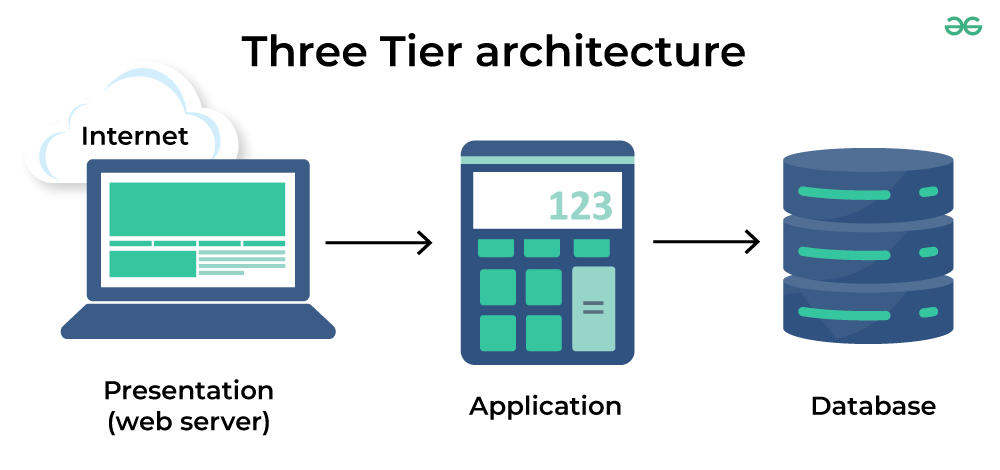
\includegraphics[width=1\linewidth]{figures/three-tier-architecture.png}
	\caption{Caption của ảnh 1}
	\label{fig:UET_logo2}
\end{figure}

% Thêm float barrier để ngăn chặn các hình ảnh tràn ra ngoài chương
\FloatBarrier


Hình ảnh được xoay dọc (với những hình ảnh có chiều ngang quá lớn, nếu để ngang chữ sẽ bị bé, bị vỡ ảnh hoặc không nhìn rõ):

\begin{figure} [!htb]
	\centering
	\rotatebox{90}{
        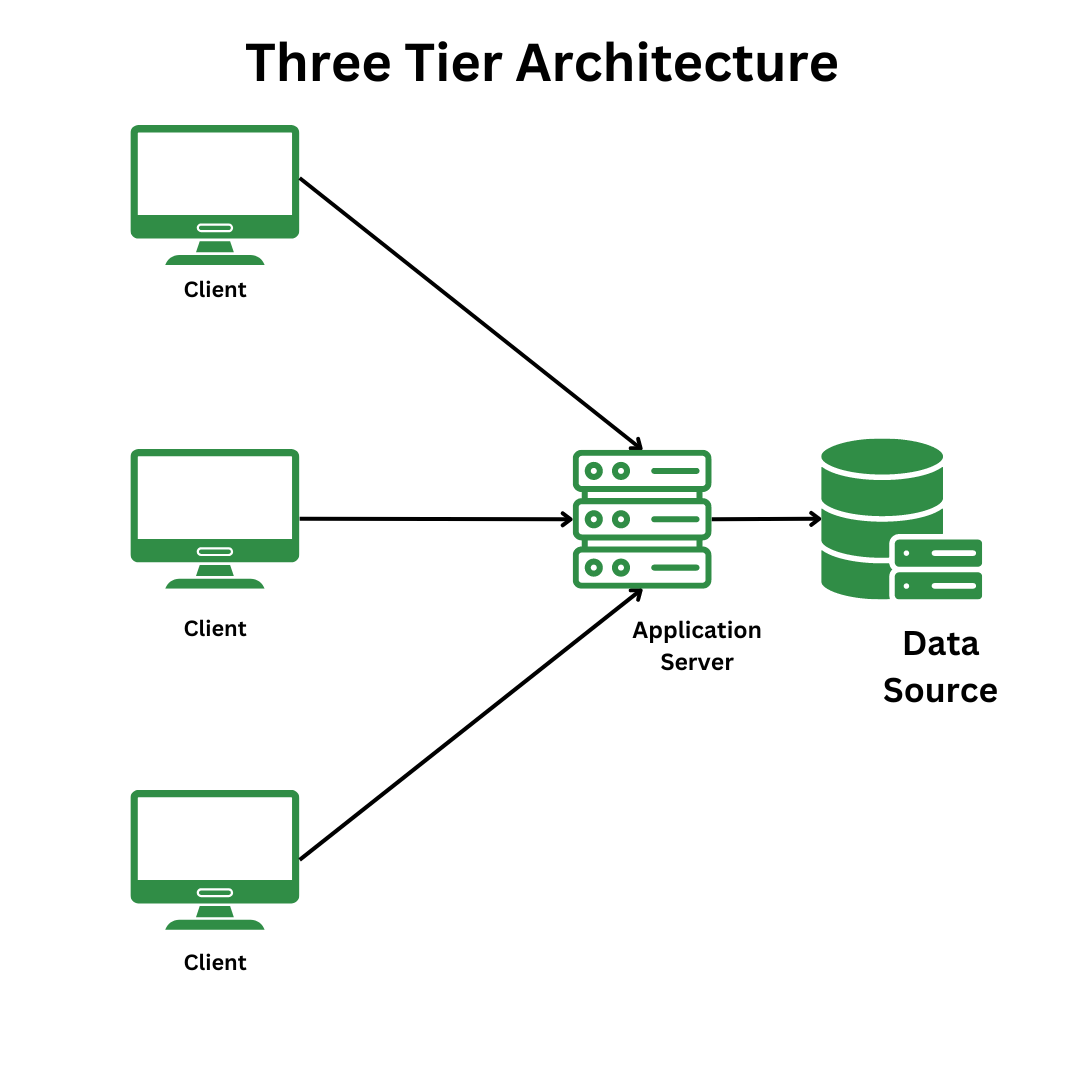
\includegraphics[width=0.5\linewidth]{figures/three-tier-architecture-2.png}
    }
	\caption{Caption của ảnh 2}
	\label{fig:UET_logo}
\end{figure}

% Thêm float barrier để ngăn chặn các hình ảnh tràn ra ngoài chương
\FloatBarrier

\vspace{1cm}

\textbf{Trích dẫn:} Các mục trích dẫn viết trong file main.tex, các trích dẫn viết theo chuẩn IEEE, khi muốn trích dẫn thì viết như này \cite{Cockburn2005}



\begin{landscape}
	\noindent Bảng biểu

	\begin{longtable}{|>{\raggedright\arraybackslash}m{4cm}|>{\raggedright\arraybackslash}m{4.5cm}|>{\raggedright\arraybackslash}m{4.5cm}|>{\raggedright\arraybackslash}m{4.5cm}|>{\raggedright\arraybackslash}m{4.5cm}|}
	\caption{Caption của bảng} \\
	\hline
	\textbf{Tính năng} & \textbf{Hệ thống} & \textbf{Đối thủ 1} & \textbf{Đối thủ 2} & \textbf{Đối thủ 3} \\
	\hline
	Tính năng 1 & x & x & x & x \\
	\hline
	Tính năng 2 & x & x & x & x \\
	\hline
	Tính năng 3 & x & x & x & x \\
	\hline
	Tính năng 4 & x & x & x & x \\
	\hline

\end{longtable}
\end{landscape}



\vspace{0.3cm}


Đoạn kết luận chương: tóm tắt lại nội dung của chương này, dẫn dắt vào nội dung chương tiếp theo.
\newpage
\clearpage
\phantomsection

\setcounter{chapter}{1}
\chapter[{Tên chương 2}]{Tên chương 2}

Đoạn giới thiệu chương.

\section{Mục lớn trong chương}

abcabc

\subsection{Mục nhỏ trong chương}

abc

\subsection{Mục nhỏ trong chương}

abc

\section{Mục lớn trong chương}

abcabc

\subsection{Mục nhỏ trong chương}

abc


\vspace{0.5cm}

Đoạn kết luận chương
\newpage
\clearpage
\phantomsection

\setcounter{chapter}{2}
\chapter[{TÊN CHƯƠNG 3}]{Tên chương 3}

\newpage
\clearpage
\phantomsection

\setcounter{chapter}{3}
\chapter[{TÊN CHƯƠNG 4}]{Tên chương 4}

% Sau khi hoàn tất quá trình phân tích và thiết kế hệ thống, chương 4 sẽ trình bày quá trình cấu hình, cài đặt và kiểm thử các tính năng của hệ thống theo kiến trúc đã đề ra. Hệ thống đã được đóng gói dưới dạng image, người dùng có thể sử dụng ứng dụng Docker để cài đặt hệ thống trên máy chủ tại chỗ của tổ chức, doanh nghiệp.

% \section{Cài đặt hệ thống}

% Để cài đặt hệ thống ServeFlow, người dùng cần chuẩn bị một máy chủ với các thông số tối thiểu như sau:
% \renewcommand{\labelitemi}{$-$}
% \begin{itemize}
%     \item \textit{CPU}: tối thiểu 4 lõi.
%     \item \textit{RAM}: tối thiểu 8 GB.
%     \item \textit{Ổ cứng}: dung lượng còn trống tối thiểu 20 GB.
% 	\item \textit{Hệ điều hành}: từ Ubuntu 20.04 trở lên
% \end{itemize} 
% \vspace{0.3cm}

% Người dùng thực hiện lần lượt các bước sau:

% \subsection{Cài đặt Docker}
% Cập nhật danh sách gói cài đặt:

% \begin{lstlisting}[language=bash, basicstyle=\ttfamily\small, backgroundcolor=\color{gray!10}]
% 	sudo apt update
% \end{lstlisting}


% Cài đặt ứng dụng docker:
% \begin{lstlisting}[language=bash, basicstyle=\ttfamily\small, backgroundcolor=\color{gray!10}]
% 	sudo apt install docker.io -y
% \end{lstlisting}

% Khởi chạy ứng dụng docker:
% \begin{lstlisting}[language=bash, basicstyle=\ttfamily\small, backgroundcolor=\color{gray!10}]
% 	sudo systemctl start docker
% 	sudo systemctl enable docker
% \end{lstlisting}

% Kiểm tra Docker đã được cài đặt:
% \begin{lstlisting}[language=bash, basicstyle=\ttfamily\small, backgroundcolor=\color{gray!10}]
% 	docker --version
% \end{lstlisting}

% \subsection{Tải về image ServeFlow}
% Image khởi chạy của ServeFlow đã được cập nhật trên kho lữu trữ Docker Hub. Người dùng sử dụng lệnh sau để tải về:
% \begin{lstlisting}[language=bash, basicstyle=\ttfamily\small, backgroundcolor=\color{gray!10}]
% 	docker pull huythai855/serveflow:latest
% \end{lstlisting}


% \subsection{Chạy container ServeFlow}
% Sau khi đã tải về image của ServeFlow, người dùng có thể chạy container với các biến môi trường và cấu hình cổng như sau:
% \begin{lstlisting}[language=bash, basicstyle=\ttfamily\small, backgroundcolor=\color{gray!10}]
% 	docker run -d \
% 	--name serveflow \
% 	-p 8000:8000 \
% 	-e MONGO_URI="mongodb://<mongo_host>:<port>" 
% 	-e POSTGRES_URI="postgresql://<host>:<port>/<db>" 
% 	-e REDIS_URL="redis://<host>:<port>"
% 	huythai855/serveflow:latest
% \end{lstlisting}

% Trong đó:
% \renewcommand{\labelitemi}{$-$}
% \begin{itemize}
% 	\item \textit{MONGO\_URI}: là thông tin kết nối đến MongoDB, ví dụ: mongodb://localhost:27017.
% 	\item \textit{POSTGRES\_URI}: là thông tin kết nối đến PostgreSQL, ví dụ: postgresql://localhost:5432.
% 	\item \textit{REDIS\_URL}: là thông tin kết nối đến Redis, ví dụ: redis://localhost:6379.
% \end{itemize}

% Sau khi container đã được khởi chạy, người dùng có thể truy cập vào địa chỉ \textit{http://localhost:8000} để sử dụng hệ thống ServeFlow.

% \vspace{0.5cm}

% \section{Hệ thống triển khai và quản lý mô hình ServeFlow}

% \subsection{Đăng nhập}

% Khi truy cập vào hệ thống, nếu kiểm tra người dùng chưa đăng nhập, hệ thống sẽ ngay lập tức chuyển hướng người dùng về trang Login. Tại đây, ở lần đầu đăng nhập, người dùng sử dụng tài khoản quản trị viên đã cấu hình khi cài đặt hệ thống để đăng nhập. Đây là tài khoản quản trị viên duy nhất, tài khoản này có mọi quyền thêm, sửa, xóa, cập nhật các mô hình và có quyền tạo mới hoặc xóa các tài khoản của những người dùng khác trong hệ thống.

% \begin{figure} [!htb]
% 	\centering
% 	\includegraphics[width=1\linewidth]{figures/gd_login.png}
% 	\caption{Giao diện đăng nhập tài khoản của hệ thống}
% 	\label{fig:RelationalDatabaseDiagram}
% \end{figure}

% \FloatBarrier



% \subsection{Trang chủ}

% Ngay sau khi đăng nhập, người dùng sẽ được chuyển hướng về trang chủ. Tại đây, hệ thống sẽ hiển thị các thông tin tổng quan nhất của hệ thống, bao gồm số lượng triển khai đang ở mỗi trạng thái, số lượng cụm đang kết nối, tổng quan số tài nguyên đang sử dụng. Từ đó, người dùng hệ thống có thể dễ dàng nắm bắt các thông tin một cách nhanh chóng.

% \begin{figure} [!htb]
% 	\centering
% 	% \rotatebox{90}{
%     %     \includegraphics[width=1.5\linewidth]{figures/image29.png}
%     % }
% 	\includegraphics[width=1\linewidth]{figures/gd_dashboard.png}

% 	\caption{Giao diện trang chủ của hệ thống}
% 	\label{fig:RelationalDatabaseDiagram}
% \end{figure}

% \FloatBarrier





% \subsection{Cảnh báo}

% Với ServeFlow, người dùng có thể cùng lúc đăng ký nhiều cụm máy chủ Kubernetes vào cùng một lúc, do đó lượng hạ tầng cần quản lý là rất nhiều. Hệ thống sẽ liên tục thu thập và giám sát thông tin về trạng thái tài nguyên, hiệu năng hoạt động và các lỗi phát sinh từ các cụm được kết nối khi phát hiện những dấu hiệu bất thường như:

% \renewcommand{\labelitemi}{$-$}
% \begin{itemize}
%     \item Cụm Kubernetes bị mất kết nối hoặc gặp sự cố xác thực.
%     \item Tình trạng tài nguyên ở các cụm vượt quá mức cấu hình.
%     \item Các deployment khi khởi tạo bị treo hoặc khởi động lại liên tục.
% \end{itemize} 
% \vspace{0.3cm}


% Khi đó, hệ thống sẽ tự động sinh các cảnh báo và ghi lại vào cơ sở dữ liệu MongoDB thực hiện việc tra cứu cũng như ngay lập tức hiển thị ở mục Cảnh báo (Alerts) cho người dùng, giúp quản trị viên hệ thống ngay lập tức có phương án điều chỉnh, xử lý sự cố ngay lập tức.


% \begin{figure} [!htb]
% 	\centering
% 	% \rotatebox{90}{
%     %     \includegraphics[width=1.5\linewidth]{figures/image3.png}
%     % }
% 	\includegraphics[width=\linewidth]{figures/gd_alerts.png}
% 	\caption{Giao diện trang cảnh báo của hệ thống}
% 	\label{fig:RelationalDatabaseDiagram}
% \end{figure}

% \FloatBarrier






% \subsection{Nhật ký hoạt động}

% Tính năng nhật ký hoạt động (Activity Log) trong ServeFlow cho phép theo dõi toàn bộ hoạt động của người dùng trong hệ thống theo thời gian thực. Do hệ thống có rất nhiều người dùng, dùng cùng một thời điểm, đây là công cụ quan trọng giúp quản trị viên giám sát, kiểm tra và truy vết các thay đổi ảnh hưởng đến hệ thống triển khai mô hình.


% Tính năng nhật ký hoạt động hỗ trợ:
% \renewcommand{\labelitemi}{$-$}
% \begin{itemize}
%     \item Đảm bảo tính minh bạch và trách nhiệm khi vận hành.
%     \item Dễ dàng truy vết nguyên nhân sự cố khi xảy ra lỗi.
%     \item Phân tích hành vi sử dụng hệ thống và phát hiện bất thường.
% \end{itemize} 
% \vspace{0.3cm}


% \begin{figure} [!htb]
% 	\centering
% 	% \rotatebox{90}{
%     %     \includegraphics[width=1.5\linewidth]{figures/image12.png}
%     % }
% 	\includegraphics[width=1\linewidth]{figures/gd_activity_logs.png}
% 	\caption{Giao diện trang nhật ký hoạt động của hệ thống}
% 	\label{fig:RelationalDatabaseDiagram}
% \end{figure}

% \FloatBarrier



% \subsection{Kho lưu trữ mẫu triển khai mô hình}

% ServeFlow cung cấp tính năng Model Template - một kho lưu trữ các mẫu triển khai mô hình được dựng sẵn (build-in). Đây là danh sách các mô hình phổ biến cho từng bài toán. Người dùng có thể tìm kiếm mô hình theo bài toán mình đang cần sử dụng, xem các thông tin mô tả, thông số, các ca sử dụng tốt nhất,... từ đó lựa chọn được mô hình phù hợp nhất để sử dụng. Các mẫu triển khai (template) đều đã có sẵn các bộ thông số triển khai, giúp người dùng khi đã chọn lựa được mô hình phù hợp với bài toán của mình, có thể ngay lập tức lựa chọn cụm Kubernetes và triển khai ngay lập tức.


% \begin{figure} [!htb]
% 	\centering
% 	\includegraphics[width=1\linewidth]{figures/gd_model_template2.png}
% 	\caption{Giao diện kho lưu trữ mẫu triển khai mô hình của hệ thống.}
% 	\label{fig:RelationalDatabaseDiagram}
% \end{figure}

% \FloatBarrier

% \begin{figure} [!htb]
% 	\centering
% 	\includegraphics[width=1\linewidth]{figures/gd_model_template_detail2.png}
% 	\caption{Giao diện xem chi tiết mẫu triển khai mô hình của hệ thống.}
% 	\label{fig:RelationalDatabaseDiagram}
% \end{figure}

% \FloatBarrier



% \subsection{Quản lý người dùng}

% Tính năng quản lý người dùng (User Management) của ServeFlow cho phép quản trị viên thêm, bớt, sửa xóa toàn bộ danh sách người dùng trong hệ thống, giúp đảm bảo bảo mật và phân quyền truy cập rõ ràng giữa các thành viên. Như đã đề cập ở phần 3.4. Tầng giao diện, người dùng hệ thống được phân thành ba nhóm vai trò: Admin, User và Observer. Mỗi nhóm vai trò sẽ có các quyền truy cập và thao tác khác nhau trong hệ thống.

% ServeFlow được xây dựng với mong muốn cung cấp một hệ thống triển khai và quản lý mô hình học máy toàn diện dành cho các nhóm nghiên cứu và doanh nghiệp. Không chỉ hỗ trợ triển khai mô hình trên hạ tầng cụm Kubernetes một cách đơn giản, ServeFlow còn nổi bật với khả năng quản trị, phân quyền người dùng rõ ràng và trực quan, tính năng mà mà nhiều giải pháp hiện tại như Triton Inference Server, Kubeflow và MLflow chưa đáp ứng và tối ưu tốt cho môi trường làm việc nhóm.


% \begin{figure} [!htb]
% 	\centering
% 	% \rotatebox{90}{
%     %     \includegraphics[width=1.5\linewidth]{figures/gd_user_management.png}
%     % }
% 	\includegraphics[width=1\linewidth]{figures/gd_user_management.png}
% 	\caption{Giao diện quản lý người dùng của hệ thống.}
% 	\label{fig:RelationalDatabaseDiagram}
% \end{figure}

% \FloatBarrier








% \subsection{Quản lý token}

% Tính năng quản lý token (Token Management) của ServeFlow cho phép người dùng tạo và quản lý các token truy cập vào hệ thống. Token là một chuỗi ký tự duy nhất được sử dụng để xác thực và phân quyền truy cập vào các tài nguyên trong hệ thống. Các token được sinh tự động, ngẫu nhiên, chỉ hiển thị lần đầu tiên khi tạo. Sau khi tạo xong, hệ thống sẽ lưu lại thông tin của token vào cơ sở dữ liệu để có thể quản lý và xác thực.

% \begin{figure} [!htb]
% 	\centering
% 	% \rotatebox{90}{
%     %     \includegraphics[width=1.5\linewidth]{figures/gd_user_management.png}
%     % }
% 	\includegraphics[width=1\linewidth]{figures/gd_user_management.png}
% 	\caption{Giao diện quản lý người dùng của hệ thống.}
% 	\label{fig:RelationalDatabaseDiagram}
% \end{figure}

% \FloatBarrier








% \subsection{Quản lý cụm Kubernetes}

% Một trong những điểm đặc biệt của ServeFlow so với các giải pháp hiện tại là khả năng quản lý nhiều cụm k8s thay vì cố định trên một nền tảng. Khả năng này cho phép người dùng linh hoạt triển khai mô hình học máy trên cả môi trường tại chỗ (on-premise) và trên các nền tảng đám mây (cloud-based). Người dùng có thể đăng ký các cụm Kubernetes tự triển khai trên server của doanh nghiệp hoặc từ nhiều nhà cung cấp cả trong nước lẫn quốc tế như FPT Cloud, Microsoft Azure, Google Cloud.

% Để thêm một cụm mới vào hệ thống, người dùng nhấn nút Register Cluster trên giao diện. Hệ thống sẽ yêu cầu người dùng cung cấp nội dung tệp kubeconfig tương ứng với cụm Kubernetes muốn kết nối. Sau khi xác thực thành công, cụm sẽ được thêm vào danh sách và trạng thái kết nối sẽ hiển thị là \textit{Connected}.


% \begin{figure} [!htb]
% 	\centering
% 	% \rotatebox{90}{
%     %     \includegraphics[width=1.5\linewidth]{figures/image14.png}
%     % }
% 	\includegraphics[width=1\linewidth]{figures/gd_cluster.png}
% 	\caption{Giao diện tính năng quản lý cụm Kubernetes của hệ thống.}
% 	\label{fig:RelationalDatabaseDiagram}
% \end{figure}

% \FloatBarrier


% \subsection{Quản lý triển khai}

% Tính năng quan trọng nhất của hệ thống chính là quản lý triển khai mô hình học máy. ServeFlow cung cấp giao diện trực quan để người dùng dễ dàng tạo mới và quản lý các deployment trên các cụm Kubernetes đã kết nối.

% Để tạo một deployment mới, người dùng nhấn vào nút vào Create Deployment và thao tác bốn bước chính:

% \renewcommand{\labelitemi}{$-$}
% \begin{itemize}
%     \item \textit{Cài đặt mô hình (model settings)}: người dùng cấu hình các thông tin như tên, mô tả deployment, thông tin model, thông tin image triển khai và lựa chọn cụm mà sẽ triển khai deployment lên.
%     \item \textit{Cài đặt deployment (deployment settings)}: Người dùng cấu hình các thông tin của deployment chạy trên cụm kubernetes như lượng tài nguyên (CPU, RAM, GPU), số lượng bản sao (replica), các biến môi trường (environment variable), lệnh khởi động (startup command),...
%     \item \textit{Cài đặt truy cập (traffic settings)}: Người dùng cấu hình cài đặt truy cập như loại traffic trong Kubernetes, các cổng (port) được mở,...
%     \item \textit{Kiểm tra lại thông tin (review)}: Người dùng rà soát lại các thông tin triển khai deployment.
% \end{itemize} 
% \vspace{0.3cm}



% \begin{figure} [!htb]
% 	\centering
% 	% \rotatebox{90}{
%     %     \includegraphics[width=1\linewidth]{figures/gd_create_deployment2.png}
%     % }
% 	\includegraphics[width=1\linewidth]{figures/gd_create_deployment2.png}
% 	\caption{Giao diện tạo deployment mới của hệ thống.}
% 	\label{fig:RelationalDatabaseDiagram}
% \end{figure}

% \FloatBarrier


% Sau khi người dùng đã tạo deployment thành công, hệ thống sẽ chuyển hướng đến giao diện danh sách các deployment đang triển khai. Tại đây, người dùng có thể xem được thông tin tổng quan của các deployment như trạng thái deployment hay lượng tài nguyên sử dụng.

% \begin{figure} [!htb]
% 	\centering
% 	% \rotatebox{90}{
%     %     \includegraphics[width=1\linewidth]{figures/gd_deployment_list.png}
%     % }
% 	\includegraphics[width=1\linewidth]{figures/gd_deployment_list.png}
% 	\caption{Giao diện danh sách deployment của hệ thống.}
% 	\label{fig:RelationalDatabaseDiagram}
% \end{figure}

% \FloatBarrier

% Người dùng có thể nhấn vào một triển khai bất kỳ để xem thông tin chi tiết của triển khai này và nhấn vào nút Edit Deployment khi muốn cập nhật thông tin, cấu hình của triển khai này.


% \begin{figure} [!htb]
% 	\centering
% 	% \rotatebox{90}{
%     %     \includegraphics[width=1.5\linewidth]{figures/gd_deployment_detail.png}
%     % }
% 	\includegraphics[width=1\linewidth]{figures/gd_deployment_detail.png}

% 	\caption{Giao diện xem chi tiết một deployment của hệ thống.}
% 	\label{fig:RelationalDatabaseDiagram}
% \end{figure}

% \FloatBarrier




% \subsection{Thử nghiệm thực tế qua giao diện}

% Một tính năng bổ sung thêm so với các nền tảng triển khai mô hình mã nguồn mở phổ biến khác như Triton Inference Server, MLflow, hay Kubeflow, hệ thống ServeFlow cung cấp một giao diện thử nghiệm trực quan và đơn giản thông qua giao diện, giúp người dùng có thể tương tác với mô hình ngay trong trình duyệt mà không cần sử dụng giao diện dòng lệnh hay phải viết mã nguồn để kết nối. Để sử dụng tính năng này, người dùng thực hiện lần lượt các bước:

% \renewcommand{\labelitemi}{$-$}
% \begin{itemize}
%     \item \textit{Lựa chọn deployment (select deployment)}: Người dùng lựa chọn đúng deployment trong danh sách các deployment đã triển khai. Lưu ý, deployment được chọn phải đang chạy, ở trạng thái Running.
%     \item \textit{Lựa chọn phương thức thử nghiệm (select test method)}: Người dùng lựa chọn phương thức thử nghiệm. Hệ thống hiện tại đang support các phương thức cơ bản: Text to Text, Text to Image, Image to Text,,...
%     \item \textit{Điền thông tin Endpoint URL}: Tùy vào image mà người dùng lựa chọn triển khai ở mỗi deployment, thông tin đầu ra URL sẽ khác nhau. Người dùng điền endpoint URL và port để hệ thống có thể gửi và nhận yêu cầu đúng địa chỉ.
%     \item \textit{Thực hiện thử nghiệm trên giao diện Test Console}: Người dùng thực hiện thử nghiệm thông qua việc nhập văn bản hoặc hình ảnh đầu vào và nhận đầu ra, tùy theo phương thức thử nghiệm đã chọn của deployment.
% \end{itemize} 
% \vspace{0.3cm}



% \begin{figure} [!htb]
% 	\centering
% 	% \rotatebox{90}{
%     %     \includegraphics[width=1\linewidth]{figures/gd_live_test.png}
%     % }
% 	\includegraphics[width=1\linewidth]{figures/gd_live_test.png}

% 	\caption{Giao diện tính năng thử nghiệm thực tế của hệ thống}
% 	\label{fig:RelationalDatabaseDiagram}
% \end{figure}

% \FloatBarrier

% % \section{Kiểm thử mô hình}

% \section{So sánh với các hệ thống đã nêu ở chương 1}

% Ta có bảng so sánh các tính năng của ServeFlow với các hệ thống đã nêu ở chương 1 như sau:




% Có thể thấy rằng, ServeFlow đã kế thừa và học hỏi được các tính năng, đồng thời khắc phục được một số nhược điểm của các hệ thống hiện tại như không có giao diện người dùng, không hỗ trợ phân quyền người dùng hay không theo dõi được trạng thái của các triển khai. Hệ thống cũng có thể mở rộng và tuỳ biến tốt hơn cho các bài toán cụ thể của doanh nghiệp. Tuy nhiên, ServeFlow vẫn còn một số hạn chế như chưa hỗ trợ đầy đủ các cơ chế cấu hình tự động mở rộng và chưa tối ưu tốt các tài nguyên sử dụng như Triton Inference Server hay Kubeflow.







% \vspace{1cm }

% Chương 4 đã trình bày chi tiết về quá trình cài đặt và kiểm thử các tính năng trong hệ thống ServeFlow. Hệ thống đã được triển khai thành công, kết nối với các cụm Kubernetes và có thể sử dụng để triển khai và quản lý các mô hình học máy một cách dễ dàng và hiệu quả. Tuy vẫn còn một số tính năng chưa được tối ưu, các tính năng cơ bản của hệ thống đã hoạt động ổn định, đáp ứng được yêu cầu đã đề ra.

\newpage
\clearpage
\phantomsection

\addcontentsline{toc}{chapter}{{Tổng kết}}
\chapter*{Tổng kết}

Đoạn 1: Bối cảnh và tầm quan trọng của bài toán.

\vspace{0.3cm}

Đoạn 2: Các kết quả đạt được.

\vspace{0.3cm}

Đoạn 3: Các mặt hạn chế.

\vspace{0.3cm}

Đoạn 4: Hướng phát triển trong tương lai.
\newpage

% \appendix
% \input{cover/phuluc}
% \def\baselinestretch{1}
% \vspace{-2cm}



\renewcommand{\bibname}{Tài liệu tham khảo}
\clearpage
\phantomsection
\addcontentsline{toc}{chapter}{{TÀI LIỆU THAM KHẢO}}
\renewcommand{\refname}{Literary works}





\begin{thebibliography}{xx}

\section*{Tiếng Anh}

\harvarditem{Singla et al.}{2025}{Singla2025}
A. Singla, A. Sukharevsky, L. Yee, M. Chui, and B. Hall, ``The State of AI: Global survey,'' {\em McKinsey}, 2025. [Online]. Available: \url{https://www.mckinsey.com/capabilities/quantumblack/our-insights/the-state-of-ai}

\harvarditem{Zhu et al.}{2017}{Zhu2017}
X. X. Zhu, D. Tuia, L. Mou, G. Xia, L. Zhang, F. Xu and F. Fraundorfer, ``Deep learning in remote sensing: A comprehensive review and list of resources,'' {\em IEEE Geoscience and Remote Sensing Magazine}, 2017, pp.~8--36.

\harvarditem{Cockburn}{2005}{Cockburn2005}
A. Cockburn, ``What's Hexagonal Architecture?,'' {\em Medium}, [Online]. Available: \url{https://alistair.cockburn.us/hexagonal-architecture}

\end{thebibliography}




\end{document}
